% !TeX program = xelatex
\documentclass{article}

% ------- Packages and Settings --------
 
% GENERAL 

%
% Load KNMI poster package
%
% 	Options:
%
%	portrait* | landscape		set poster orientation
%	cmyk* | rgb		 	set pdf colour mode
% 	english* | dutch			set KNMI logo language
% 	epslogo* | pdflogo		set KNMI logo format
% 	disablefonts			disable all custom fonts (and the need for XeLaTeX)
% 	path			 		specify path to ?KNMIposter? (default = current directory)
% 	fixfooter			 	fix footer spacing (required for some Tex/Postscript versions)
% 	debug			 	enable geometry showframe
%
% * = default
%
\usepackage[landscape]{KNMIposter}


% USER PACKAGES
% language
\usepackage[english]{babel}

% Define path for figures -- for safety, keep the last /
\graphicspath{{example_figures/}}

% Assist LaTeX in hyphenation
\hyphenation{Rey-nold}
\hyphenation{Ra-ma-swa-my}



% Define path for figures -- for safety, keep the last /
\graphicspath{{EGU_figures/}}

% Assist LaTeX in hyphenation
\hyphenation{Rey-nold}
\hyphenation{Ra-ma-swa-my}

\usepackage{tcolorbox}
%\hypersetup{draft}
\hypersetup{colorlinks=true, citecolor=red}

\usepackage{csquotes}
% \usepackage[bibstyle=authoryear,citeystyle=numeric,firstinits=true]{biblatex}
%\usepackage[style=numeric,firstinits=true,sorting=none]{biblatex}
%\renewbibmacro{in:}{}

% ------- POSTER HEADER --------

% Poster title
\title{Automatic fog detection for public safety by using camera images}

% Author
\author{Giuliano Andrea Pagani\affil{1}, Martin Roth\affil{1}, and Wiel Wauben\affil{1}. Contact: pagani@knmi.nl}

% Affiliations
\affiliations{\affil{1}R\&D Department of Observations and Data-Technology, Royal Netherlands Meteorological Institute. PO Box 201, 3730 AE De Bilt, The Netherlands.%
}

% You can either add the contact information in the author line (poster top, large),
% or in the affiliations (poster bottom, footnote size).

% Some additional space for acknowledgements, url's, ... 
% \acknowledge{I would like to thank all of you!}


% ------- Document start --------
\begin{document}

\maketitle

\begin{abstract}
\begin{multicols}{2}
Visibility is traditionally measured manually by meteorological observers using landmarks at known distances in
the vicinity of the observation site. 
Visibility sensors are also used, but they are rather costly and
require regular maintenance. Moreover, observers, and in particular sensors, give only visibility information that is
representative for a limited area. 
Cameras are more and more deployed for surveillance and security reasons in cities and for monitoring traffic along
main transportation routes. In addition to this primary use of cameras, we consider cameras as potential sensors to
automatically identify low visibility conditions. 
The approach that we follow is to use machine learning techniques
to determine the presence of fog or to make an estimation of the visibility. 
\end{multicols}
\end{abstract}

\bcols %% Start columns

\section*{Motivation}
Fog and reduced visibility have considerable impact on the performance of road, maritime, and aeronautical transportation
networks. The impact ranges from minor delays to more serious congestions or unavailability of the
infrastructure and can even lead to damage or loss of lives~\cite{gultepe2007fog}.

%\vspace{-0.5cm}
\begin{minipage}[b]{\columnwidth}
	\begin{center}
	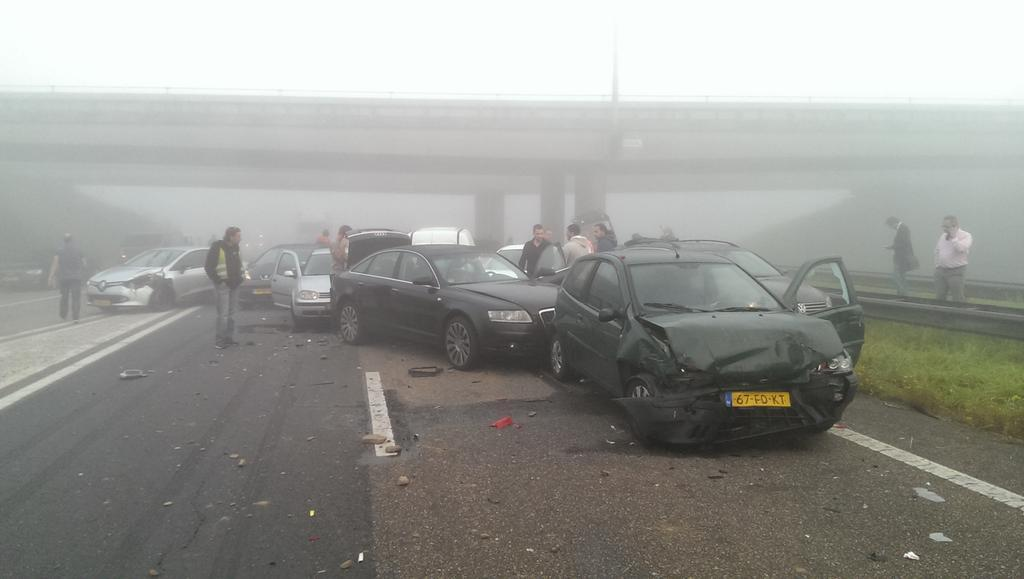
\includegraphics[width=0.9\columnwidth]{Accident.jpeg}
	\captionof{figure}{Traffic accident caused by dense fog.}
	\label{figAccident}
	\end{center}
\end{minipage}
\vspace{-2cm}

\subsection*{Key facts about fog:}
\begin{itemize}
  \item May form and dissipate suddenly.
  \item Often only a local phenomenon.
\end{itemize}

\subsection*{Limitations of current technology:}
\begin{itemize}
\item Weather stations observe a limited area.
\item Satellites are not constantly observing areas of interest.
\item Forecast of fog conditions is complex.
\end{itemize}

\subsection*{Idea:}
Use cameras deployed for surveillance and security reasons in cities and for monitoring traffic along
main transportation routes as potential sensors to
automatically identify low visibility conditions.


\begin{minipage}[b]{\columnwidth}
\centering
\begin{minipage}[b]{0.4\columnwidth}
	\begin{center}
	%\vspace*{-4mm}
	 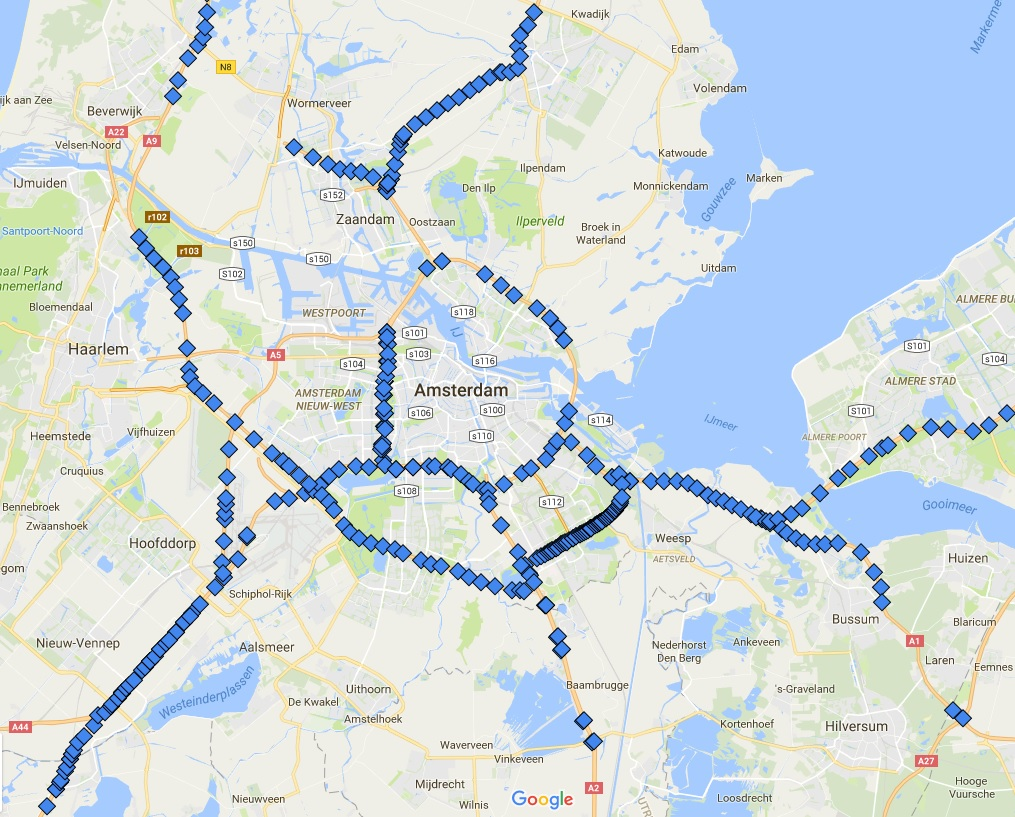
\includegraphics[width=\columnwidth]{CameraPlacement}\vspace*{1.4cm}
	\captionof{figure}{Cameras monitoring highways in Amsterdam region.}
	\label{figCameras}
	\end{center}
	\end{minipage}
	\hspace*{0.1cm}	
\begin{minipage}[b]{0.4\columnwidth}
	\begin{center}
	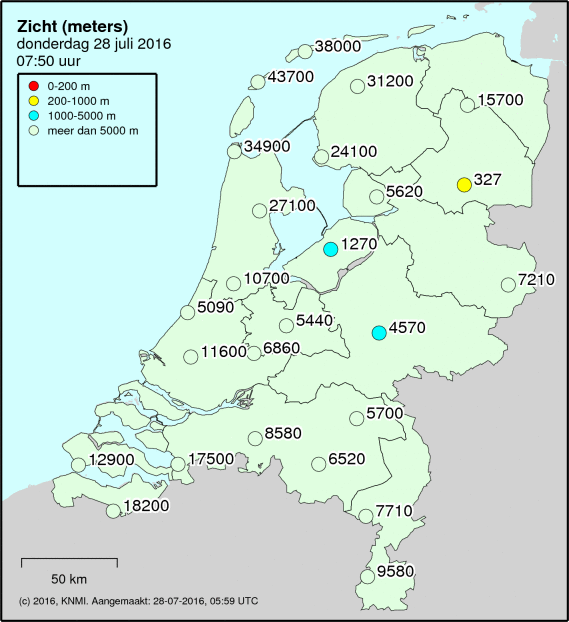
\includegraphics[width=\columnwidth]{SensorPlacement}
	\captionof{figure}{KNMI weather stations measuring visibility.}
	\label{figSensors}
	\end{center}
\end{minipage}
\end{minipage}

\section*{Approach}
% \subsection*{From Images to Machine Learning}
General properties of the images (\textbf{features}) are computed. 
Properties that are expected to vary with visibility conditions are:

\begin{tcolorbox}[colback=red!5!white,colframe=red!75!black,title=Image Features]
\begin{description}
\item[Mean Edges:] More edges indicate better visibility.
\item[Mean Brightness:] Perception of the luminance of sources of radiating/reflecting light.
\item[Mean Saturation:] The purest (most saturated) colors are obtained in the absence of atmospheric turbidity.
\item[Mean HUE:] Perception of a source of being similar to red, blue, green, yellow colors.
\item[Fractal Dimension:] Self similarity of the picture~\cite{xion14}.
\item[Transmission smoothness:] Transmission of the dark channel of the image.
\item[Transmission changepoint:] Horizontal point where the transmission of the dark channel is subject to change.
\item[Mean transmission:] Transmission of the dark channel of the image increases with visibility.
\end{description}
%\item{Weather based:}
%\begin{itemize}
%\item{Wind speed}
%\item{Dew point}
%\item{Humidity}
%\item{Precipitation amount}
%\end{itemize}
%\end{itemize}
\end{tcolorbox}


%Pictures are translated to a set of quantities capturing their properties (\textbf{features}).\newline
The measurements obtained by a nearby forward scatter sensor is considered the
reference for the visibility conditions \emph{in the measurement field}
(\textbf{supervised} problem).\newline
A classifier is trained with the features extracted from the images and the 
visibility (class) provided by the sensor.
\vspace*{0.8cm}

\textit{Restrictions}: 
i) static cameras,
ii) daylight conditions,
iii) period: 3/2015 - present, 
iv) image sampling time: 10 minutes,
see also \cite{Wauben.Roth2016}.




\begin{minipage}[b]{\columnwidth}
	\begin{center}
	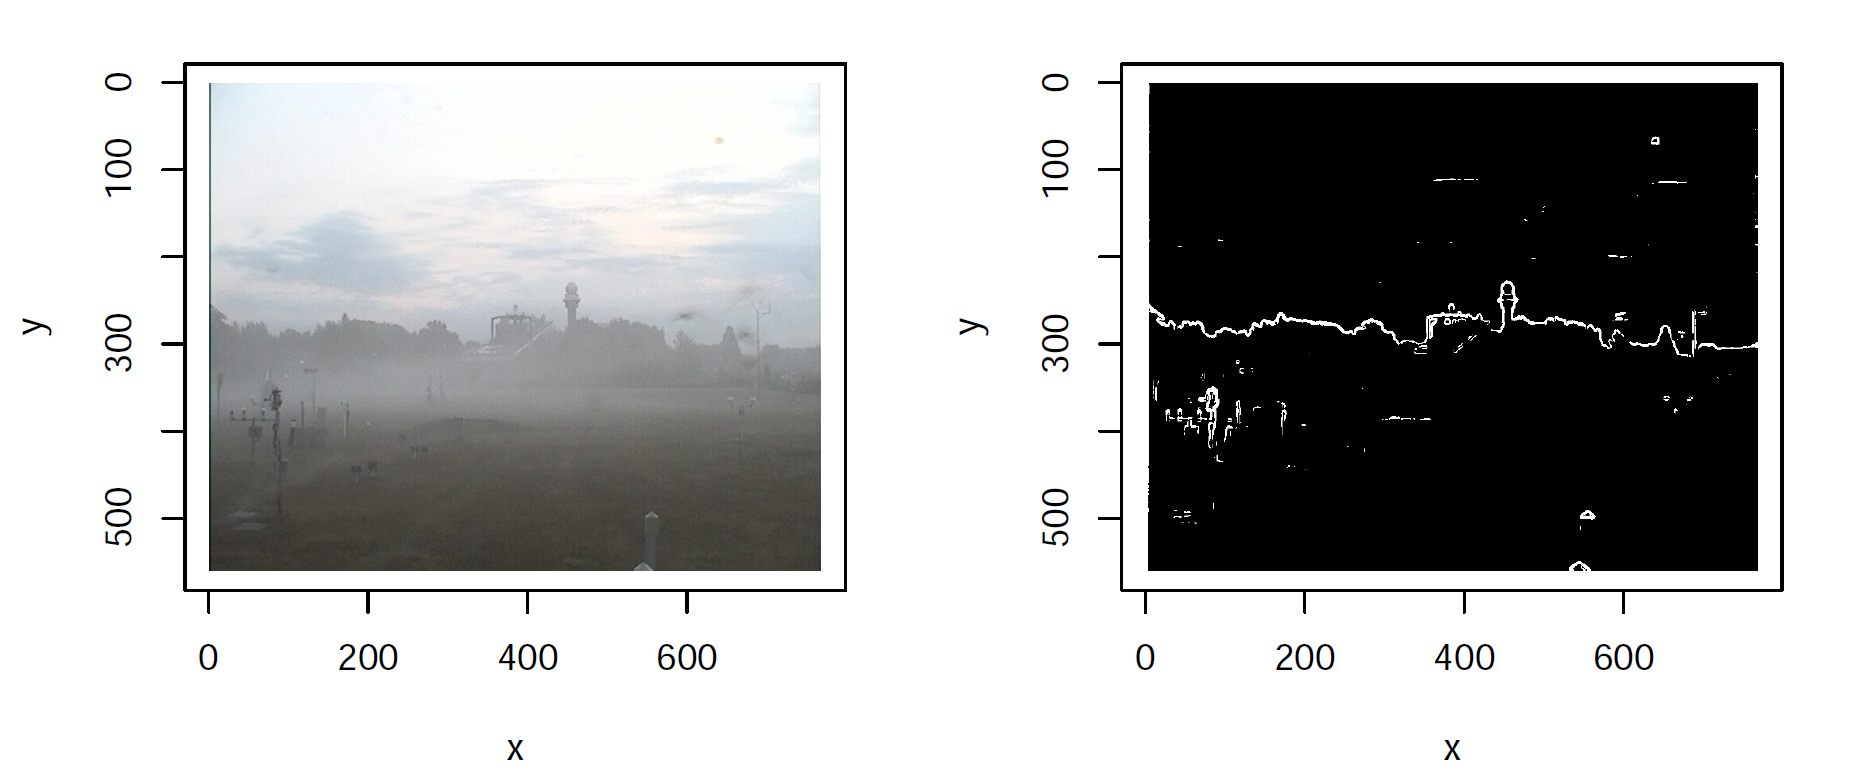
\includegraphics[width=0.95\columnwidth]{edges}
	\captionof{figure}{Image from De Bilt and corresponding edges.}
	\label{figEdges}
	\end{center}
\end{minipage}

\begin{minipage}[b]{\columnwidth}
	\begin{center}
	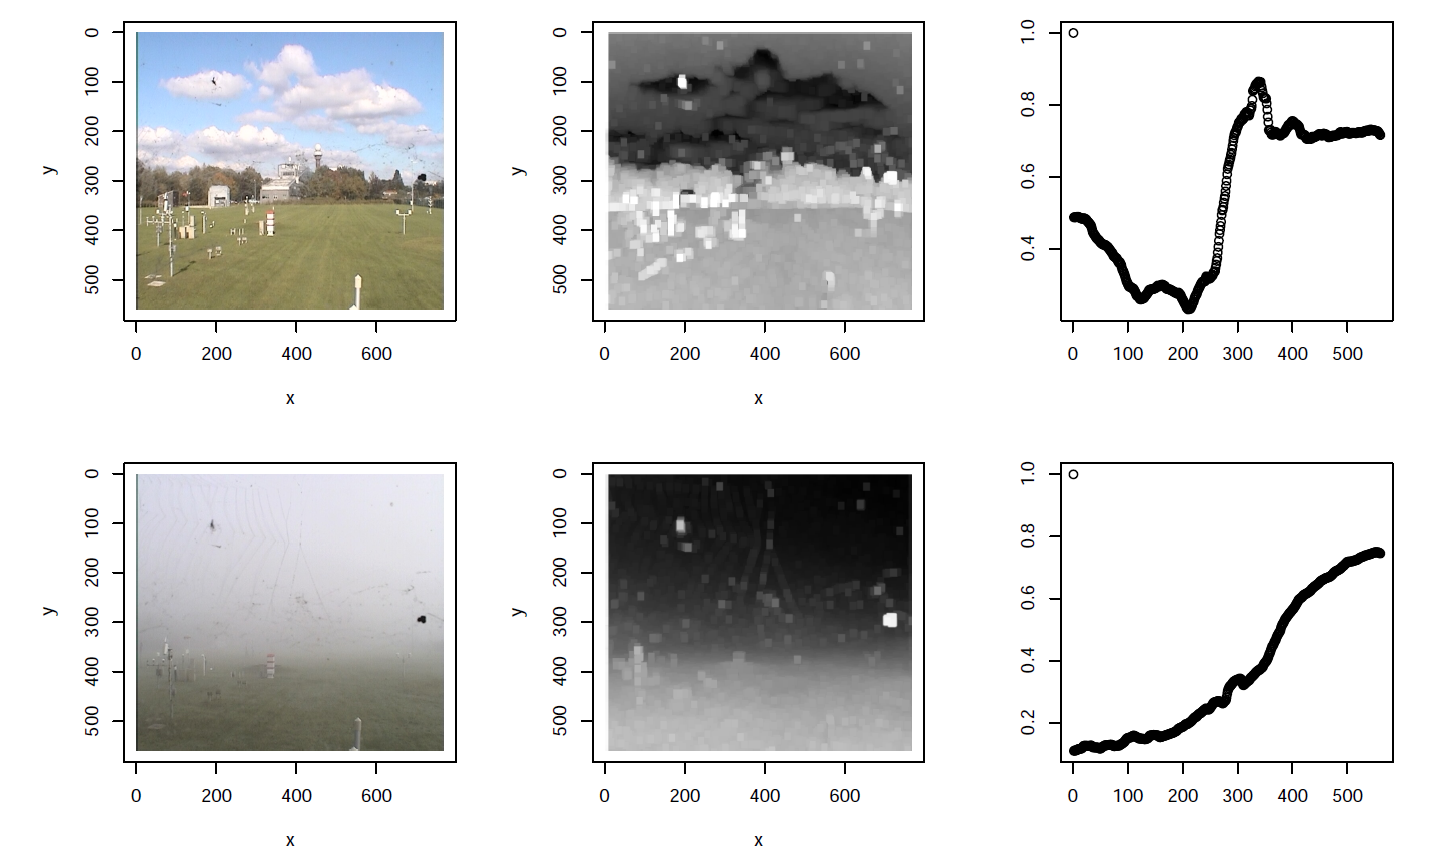
\includegraphics[width=0.95\columnwidth]{transmission}
	\captionof{figure}{Dark channel transmission and its horizontal average on a 
	  clear (top) and on a foggy (bottom) day.}
	\label{figTransmission}
	\end{center}
\end{minipage}
%\vspace*{-5cm}


\section*{Results}
The features selected to identify fog conditions from images can be visualized in a \textbf{Decision Tree}. 
This is an first exploratory approach and we aim to identify fog in more advanced and complex dynamic scenarios.

\begin{minipage}[b]{\columnwidth}
	\begin{center}
	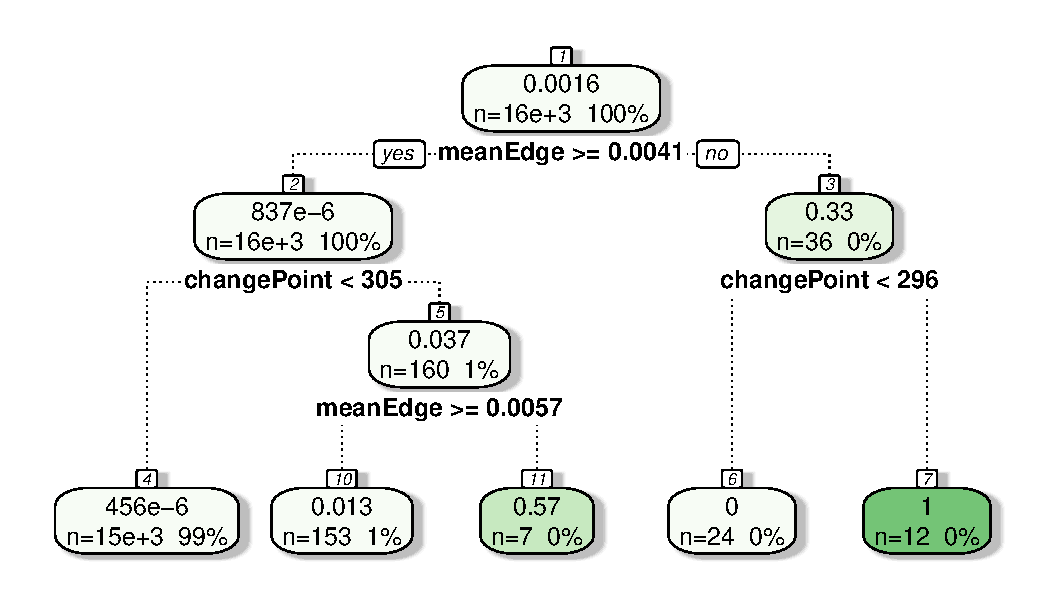
\includegraphics[width=0.9\columnwidth]{ClassificationTree-1}
	\captionof{figure}{Decision Tree results for De Bilt training set.}
	\label{figTree}
	\end{center}
\end{minipage}


\begin{tcolorbox}[colback=red!5!white,colframe=red!75!black,title=Overall Project Results]
\begin{itemize}
\item{Partnership with governmental institution for road management.}
\item{Solved privacy issues and started building image archives for analysis.}
\item{Access to traffic monitoring cameras on Dutch highways and airports.}
\item{Access to observation cameras in Dutch airports.}
\item{Processing of images in distributed infrastructure.}
\item{R package for feature calculation\\ \url{https://github.com/MartinRoth/visDec}}
\end{itemize}
\end{tcolorbox}

\begin{minipage}[b]{\columnwidth}
	\begin{center}
	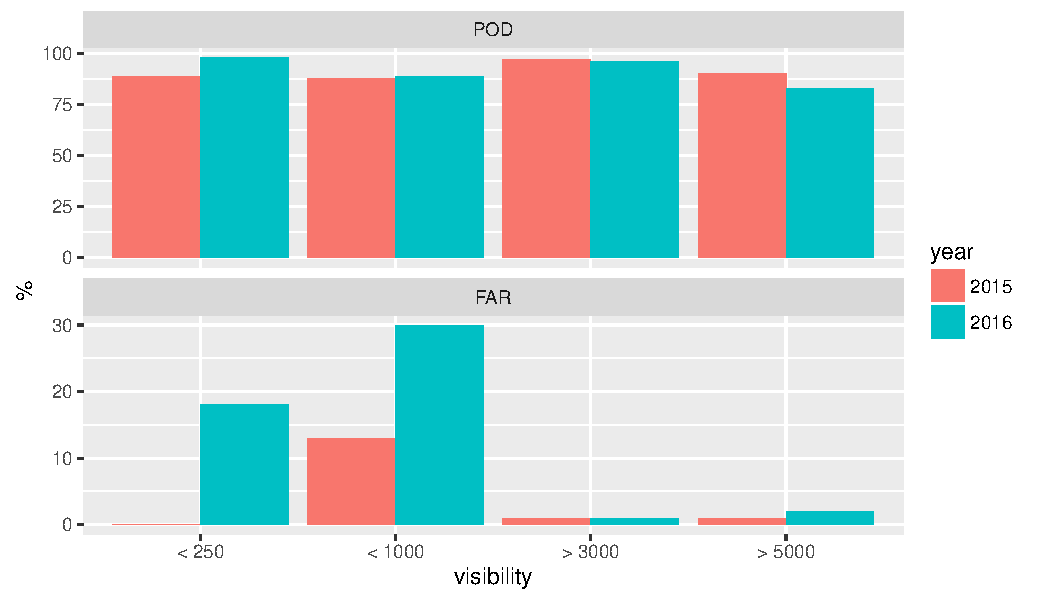
\includegraphics[width=0.85\columnwidth]{PODandFAR3-1}
	\captionof{figure}{POD-FAR for De Bilt training (2015) and test (2016)}
	\label{PODFAR}
	\end{center}
\end{minipage}
For results for location De Bilt are promising in the training 
(March-December 2015) and the test set (January-June 2016) in terms of 
\textbf{Probability of Detection} (POD) and \textbf{False Alarm Ratio} (FAR).

%\columnbreak % force jump to next column

\vspace*{-.5cm}
\section*{Follow up - Open Questions}
There are plenty of aspects we are working or planning to work on:
\begin{enumerate}
\item Analyze images from more locations. \newline
Cameras at other KNMI locations have been used. More locations are now available at airports and highways.
\item Usage of meteorological variables in addition to image features.\newline
Some initial investigations have been performed in adding meteorological conditions and having a more broad feature space.
\item Consideration of spatial and temporal relationship in the fog estimation.
\item Using an image-based approach during dawn or even night conditions? 
\item Generalization of static cameras approach to a dynamic and even totally different scenes? \emph{Master student project in collaboration with University of Amsterdam to test wether certain types of NN~\cite{ganin2016domain} can be used for this purpose.}
\end{enumerate}


% Figure
% \vspace{20pt plus 10pt minus 5pt}
% \begin{minipage}[b]{\columnwidth}\begin{center}
% 	\begin{center}
% 	\includegraphics[width=\columnwidth]{fig2}
% 	\captionof{figure}{Part of an AVIRIS flight line acquired over the Pacific Ocean. Left half: a water cloud (Sc), right half: an ice cloud (Ci).}
% 	\label{fig2}
% 	\end{center}
% \end{center}\end{minipage}


%\pushdown



\bibliographystyle{ieeetr}
\vspace*{-1.2cm}

\begin{footnotesize}
\bibliography{biblio.bib}

\end{footnotesize}


\end{multicols*} %% End columns

\end{document}
